\newslide
\section{ Some excerptes from code }
\subsection{ Structure of the class Driver }
\hrulefill \\
\begin{small}
\begin{verbatim}
void Driver::SolveNewmarkMethod(OutResultUnverg * ptUnverg)
{ 
 ptgrid=new Grid<Point2D>(ptFileType); // initialize grid for domain 

 ptUnverg->Grid(ptgrid); // print information about grid in
                          // unverg-file 

 ptAPDE=new AcousticPDE(...ptGrid, ptMaterial, ptFileType); // 

 for (step=0; step<=numsteps; step++)
  {
     ptAPDE->SolveNewmarkMethodStatic(time);

     ptUnverg->OutputResult(ptAPDE->solution());
  }
  
}
\end{verbatim}
\end{small}
\hrulefill
\newpage
\newslide
\subsection { Details of implementation of class AcousticPDE}
\hrulefill
\begin{small}
\begin{verbatim}
\\ Constructor
AcousticPDE::AcousticPDE(Grid<Point2D> * ptgrid, Material * aptMaterial,
                         FileType * aptFileType, ...)
:PDE(aptFileType,aptMaterial)
 // in PDE we initialize pointer to input file
 // and pointer to file with material data
{
    // set time function 
   ptTimeFunc=new TimeFunc(aptFileType); 
     // read material info
   ptMaterial->ReadDensityAndCompress(density,compress); // read material info
   
   ...
   ptWork=new WorkWithSysMat<Point2D, Matrix<Double> >(ptGrid);
 
   ptWork->AssembleSysMatrix(CoefLaplace,CoefMass);
   ptWork->SetRHS();
 
   ptWork->SetNodesBoundaryCondition(aptFileType);
   ptWork->SetDirichletBoundaryCondSysMat_PenaltyMethod();
}
\end{verbatim}
\end{small}
\hrulefill
\newslide
\newpage
\hrulefill
\begin{small}
\begin{verbatim}
void AcousticPDE::SolveStatic_NewmarkMethod(const Double time, const Double dt)
{
   CalcParamForNewmarkMethod(dt);  

   Boolean NeedRestore=FALSE;
   Double valueTF=ptTimeFunc->TimeFuncAtTime(time);
 
   if (valueTF==0)
     { NeedRestore=TRUE;
       ptWork->SetDirichletBoundaryCondZero_Cut();
     }
   else
     ptWork->SetDirichletBoundaryCondRHS_PenaltyMethod(valueTF);
 
   ptWork->CG(100, Jacobi);
 
  if (NeedRestore) ptWork->Restore();
 
  ... calculation of first and second derivatives of solution

  ... calculation of vectorM
 
   ptWork->SetRHS(VectM);

  solution=ptWork->getSolution();
}
\end{verbatim}
\end{small}
\hrulefill
\newpage
\newslide
\subsection{ Details of implementation of class WorkWithSysMatrix  }
\hrulefill
\begin{small}
\begin{verbatim}
 template<class Dim, class T_Matrix>  
 template <class typeBaseForm>
 void Assemble<Dim,T_Matrix>::AssembleGlobal(T_Matrix & Mat,BaseElem *) 
{
  typeBaseForm oElemMatrix(ptElem,1);  

  Dim * ptCoord=new Dim[numnodeelem]; // Dim: Point2D or Point3D  

  for (numelem=0; numelem<maxnumelem; numelem++) // loop over all elements
  {
    ptgrid->GetConnection(connection,numelem);
    ptgrid->GetCoordOfNodesElem(numelem,ptCoord); 
 
     for (ii=0; ii< MaxNumNodeElem; ii++)
         for (iii=0; iii< MaxNumNodeElem; iii++)
           {
            irow=connection[ii];
            icln=connection[iii];
            Mat(irow-1,icln-1)+=elemmat[ii][iii]; 
           }
  }
} 
\end{verbatim}
\end{small} 
\hrulefill
\newpage
\newslide
\hrulefill
\begin{small}
\begin{verbatim}
template<class Dim, class T_Matrix>
void Assemble<Dim,T_Matrix>::AssembleSysMatrix(const Double CoefL, const Double
CoefM)
{
  if (!IsCalcS) { 
                   AssembleGlobal< LaplaceInt<Dim> >(S); // S and M are stored
                   IsCalcS=TRUE;                       // in data of this class
                }
  if (!IsCalcM) {
                   IsCalcM=TRUE;
                   AssembleGlobal< MassInt<Dim> >(M);
                }
  if (CoefM!=1.0) A+=M*CoefM;
      else A+=M;
 
  if (CoefL!=1.0) A+=S*CoefL;
      else A+=S;

}
\end{verbatim}
\end{small}
\hrulefill
\newslide
\newpage
\hrulefill
\begin{small}
\begin{verbatim}
void SetRHS(const Vector<Double> & CoefM=Vector<Double>(),
            const Vector<Double> & CoefS=Vector<Double>(),
            const Vector<Double> & f=Vector<Double>());

 template<class Dim, class T_Matrix>
void Assemble<Dim, T_Matrix>::SetRHS(const Vector<Double> & CoefM,
                const Vector<Double> & CoefS, const Vector<Double> & f)
{
  if (!CoefM.size() && !CoefS.size() && !f.size()) b.Init();
  if (CoefM.size()) b=M*CoefM;
  if (CoefS.size())
                      if (CoefM.size()) b+=S*CoefS;
                         else b=S*CoefS;
  if (f.size()) if (!CoefM.size() || !CoefS.size()) b+=f;
                        else b=f;
}
\end{verbatim}
\end{small}
\hrulefill
\newpage
\newslide
\hrulefill
\begin{small}
\begin{verbatim}
template <class T_Matrix>
class SystemMatrix
{
protected:
   T_Matrix A; // system matrix

   ...
}

template< class Dim, class T_Matrix>
class WorkWithSysMat: virtual public Assemble<Dim,T_Matrix>,
                      virtual public LinSystem<Double, T_Matrix>;
\end{verbatim}
\end{small}
\hrulefill
\newpage
\newslide
\subsection{ Details of implementation of class Matrix }
\begin{figure}[H]
\begin{center}
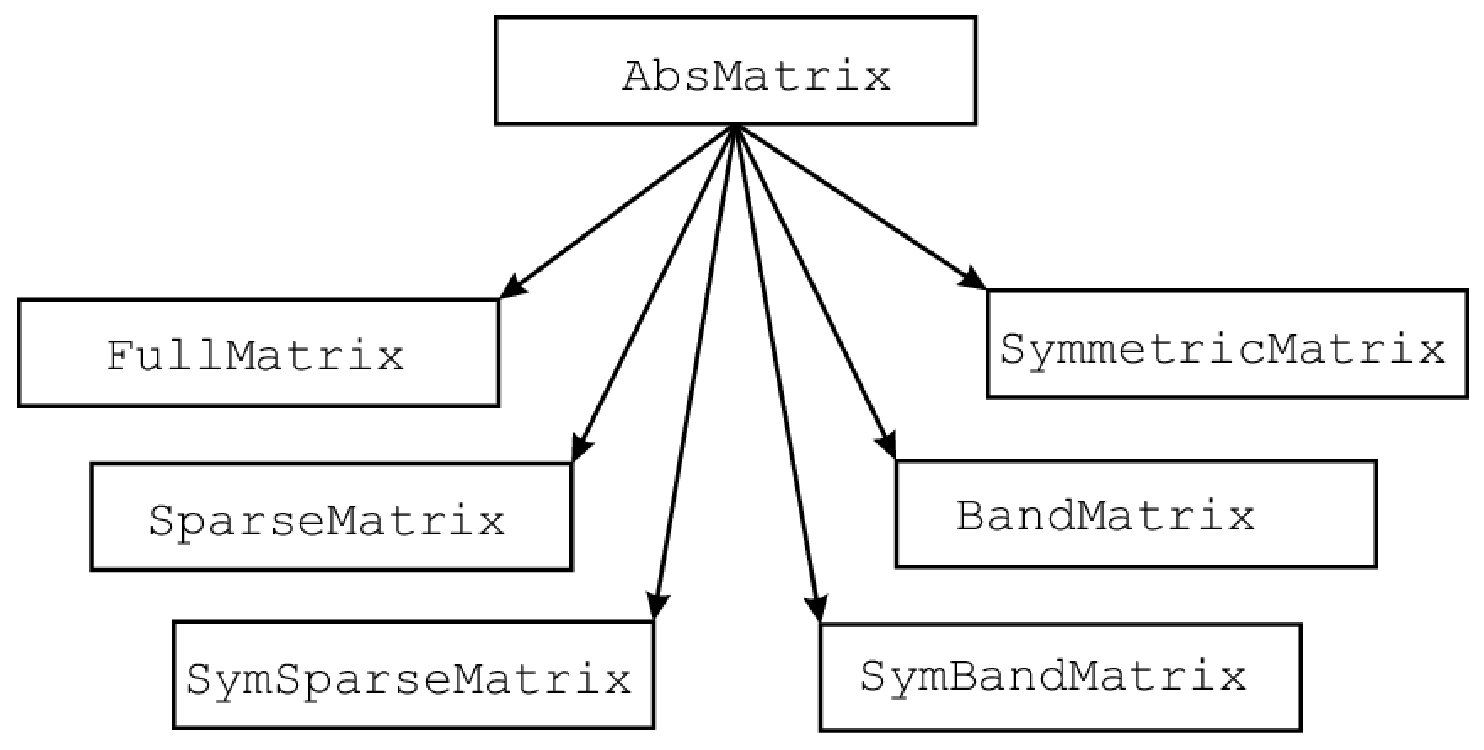
\includegraphics [width=8cm, angle=0] {./pic/Matrix1}
\end{center}
\caption{ Classes, which are derived from base class AbsMatrix } 
\end{figure}
\begin{print}
 Use of mechanism of virtual function for the implementation of the inheritance-hierarchy for different types of matrices can ruin any algorithm, because the virtual functions are called too often. Good solution for this problem is approach "recursive template". The trick is that the base class takes a template parameter, which is the type of the leaf class. So at compile time complete type of an objet is known. In this approach , leaf classes can have methods which are unique to the leaf class, and at the same time we can have default implementations of some methods. \\ 
\end{print}
% 
\newpage
\newslide
\hrulefill
\begin{small}
\begin{verbatim}
template<class T_leaftype, class TYPE>
class AbsMatrix
{
public:
   T_leaftype & asLeaf()
   { return static_cast<T_leaftype&>(*this); }
 
  Integer getSize() { return asLeaf.GetSize();}
 
  Boolean IsSymmetric() { return FALSE;}
};

template<class TYPE>
class Matrix: public AbsMatrix<Matrix<TYPE> , TYPE>; 

// Example routine which takes any matrix type
template< class T_leaftype, TYPE>
TYPE Spur(AbsMatrix<T_leaftype,TYPE> A);

\end{verbatim}
\end{small}
\hrulefill
